\subsection{Mass Parabolas of Isobars}
Isobars have the same number of nucleons (A).
\begin{align}
M(A,Z) &= Z(\overbrace{m_p + m_e}^{M(_{}^{1}H_{})}) + (\underbrace{A-Z}_{\text{neut. num.}})m_n - B(A,Z) /c^2 \\
B(A,Z) &= a_vA - a_sA^{2 / 3} - a_c\frac{Z(Z-1)}{A^{1 / 3}} - a_a\frac{(A-2Z)^2}{A} + \delta(A,Z)
\end{align}
\subsubsection{Finding the Minimum of the Mass Parabola}
As the parabola is mass $M$ as a function of $Z$, we can find the minimum by taking the derivative with respect to $Z$ and setting it equal to zero.
\begin{align}
\frac{∂ M}{∂ Z} &= 0 \\
Z_{\text{min}} &= \frac{(m_n - m_p - m_e)+a_cA^{-1 / 3} + 4a_{\text{sym}}}{2a_{c} A^{-1 / 3} + 8a_{\text{sym}}A^{-1}}
\end{align}
We can approximate this as the following:
\begin{equation}
Z_{\text{min}} ≈ \frac{A}{2} \frac{1}{1 + \frac{1}{4}A^{2/3}a_c / a_{\text{sym}}} \quad , \quad  a_{\text{sym}} ≈ 23 \text{ MeV} \ , \ a_c ≈ 0.72 \text{ MeV}
\end{equation}

\paragraph{Example: A = 10}
This is stable for smaller nuclei. 
\begin{equation}
Z_{\text{min}} ≈ 5 \quad \text{ and } \quad  \frac{Z_{\text{min}}}{A} ≈ 0.5
\end{equation}

\paragraph{Example: A = 200}
A lower ratio is stable for larger nuclei.
\begin{equation}
Z_{\text{min}} ≈ 79 \quad \text{ and } \quad  \frac{Z_{\text{min}}}{A} ≈ 0.4
\end{equation}

\subsubsection{Valley of (beta) stability}
\begin{itemize}
    \item As can be seen in \cref{fig: valley_beta_stability}, we have two parabolas for $A = 128$ as it can be odd-odd or even-even. Higher binding energy is more stable.
    \item The even-even isobar is more stable as explained in \cref{sssec: Explenation of the Terms in the Semi-Empirical Mass Formula}, because the nucleons can pair up in the same space-state with opposite spins and therefore be closer to each other and thus more stable.
    \item Only the atom in the bottom of the valley is stable. The others are prompt to beta decay downwards. 
    \item Double beta decay can happen with even numbers of nucleons as can be seen for $A = 128$ with $Z = 52$, as $Z = 53$ has higher energy, and it is therefore forced to decay all the way up to $Z = 54$. 
\end{itemize}
\begin{figure}[h!]
\centering
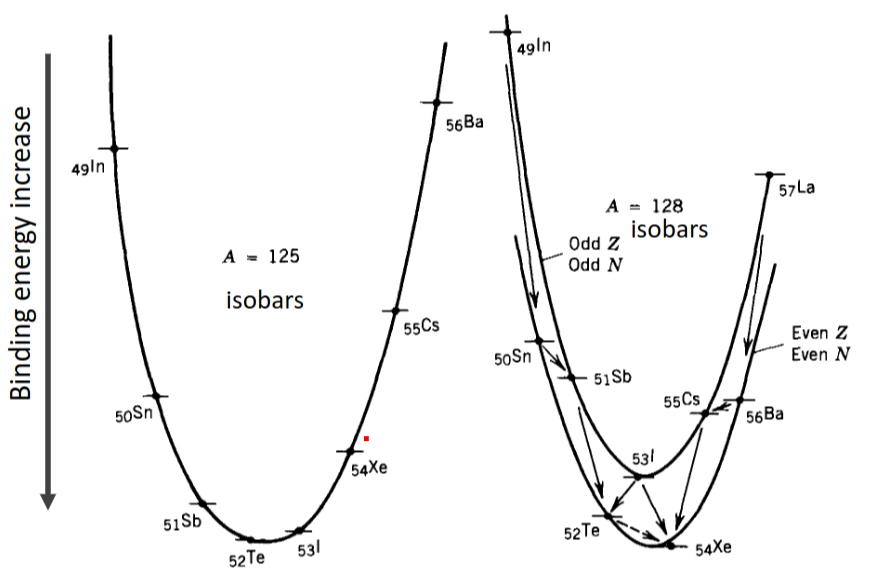
\includegraphics[width = .6\textwidth]{valley_beta_stability.png}
\caption{Valley of (beta) stability for different isobars with $A = 125$ and $A = 128$. The higher the binding energy, the more stable the isobar.}
\label{fig: valley_beta_stability}
\end{figure}

\paragraph{Beta Decay}
\begin{itemize}
    \item $β+$: Proton rich nuclei decay by converting a proton into a neutron, a positron and a neutrino. 
    \item $β-$: Neutron rich nuclei decay by converting a neutron into a proton, an electron and an antineutrino.
\end{itemize}
\begin{figure}[h!]
\centering
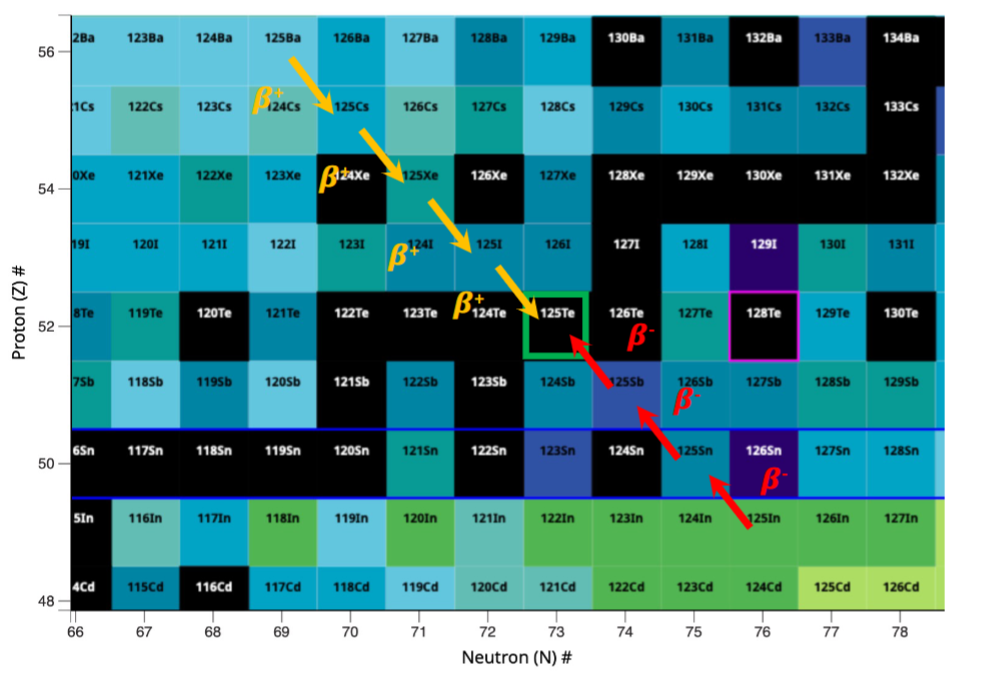
\includegraphics[width = \textwidth]{bet_decay_chart.png}
\caption{Chart showing different elements and their decays.}
\label{fig: bet_decay_chart}
\end{figure}


